% !TeX program = xelatex
\documentclass[a4paper,10pt]{article}

% ============================================================================
% សន្លឹកកិច្ចការសិស្ស ស-ខ្មៅ (Student Guided-Inquiry Worksheet - Grade 8 15.2 CIRC2)
% បរិបទ៖ គ្មានស្លាយ LCD — សិស្សប្រើរ៉ាប់ព័រទ័រវាស់ និងបំពេញតារាងសមាមាត្រទ្វេលើសន្លឹកកិច្ចការ
% វិធីសាស្ត្រ៖ POGIL + Double-Scale Proportional Ratio-Table Worksheet
% ============================================================================
\usepackage[a4paper, left=1.0cm, right=1.0cm, top=0.80cm, bottom=1.00cm, footskip=0.50cm]{geometry}
\usepackage{amsmath, amssymb}
\usepackage{unicode-math}
\usepackage{fontspec}
\usepackage{array, colortbl}
\usepackage[table]{xcolor}
\usepackage{enumitem}
\usepackage{pifont}
\usepackage{fancyhdr}
\usepackage{lastpage}
\usepackage{tikz}
\usepackage[most]{tcolorbox}
\usetikzlibrary{calc, arrows.meta, angles, quotes, decorations.markings, positioning, babel}

\makeatletter
\let\@expl@@@mark@update@singlecol@structures@@\relax
\makeatother

\providecommand{\NGSFindFonts}{%
  \IfFileExists{C:/Windows/Fonts/cambria.ttc}{%
    \def\NGSSysPath{C:/Windows/Fonts/}%
    \def\NGSUserPath{C:/Users/KIT/AppData/Local/Microsoft/Windows/Fonts/}%
  }{%
    \IfFileExists{./fonts/KhmerOSsiemreap.ttf}{\def\NGSSysPath{./fonts/}\def\NGSUserPath{./fonts/}}{%
    \IfFileExists{../fonts/KhmerOSsiemreap.ttf}{\def\NGSSysPath{../fonts/}\def\NGSUserPath{../fonts/}}{%
    \IfFileExists{../../fonts/KhmerOSsiemreap.ttf}{\def\NGSSysPath{../../fonts/}\def\NGSUserPath{../../fonts/}}{%
    \IfFileExists{../../../fonts/KhmerOSsiemreap.ttf}{\def\NGSSysPath{../../../fonts/}\def\NGSUserPath{../../../fonts/}}{%
    \IfFileExists{../../../../fonts/KhmerOSsiemreap.ttf}{\def\NGSSysPath{../../../../fonts/}\def\NGSUserPath{../../../../fonts/}}{%
    \IfFileExists{../../../../../fonts/KhmerOSsiemreap.ttf}{\def\NGSSysPath{../../../../../fonts/}\def\NGSUserPath{../../../../../fonts/}}{%
    \IfFileExists{../../../../../../fonts/KhmerOSsiemreap.ttf}{\def\NGSSysPath{../../../../../../fonts/}\def\NGSUserPath{../../../../../../fonts/}}{%
      \def\NGSSysPath{../../../../../../../fonts/}\def\NGSUserPath{../../../../../../../fonts/}%
    }}}}}}}%
  }%
}
\NGSFindFonts

\setmathfont[Path={\NGSSysPath}, FontIndex=1, Scale=1.02]{cambria.ttc}
\defaultfontfeatures{Ligatures=TeX}

\setmainfont[
  Path={\NGSUserPath}, Extension=.ttf, Script=Khmer,
  BoldFont={KhmerOSsiemreap}, BoldFeatures={FakeBold=1.8},
  ItalicFont={KhmerOSsiemreap}, ItalicFeatures={FakeSlant=0.25},
  BoldItalicFont={KhmerOSsiemreap}, BoldItalicFeatures={FakeBold=1.8, FakeSlant=0.25}
]{KhmerOSsiemreap}

\newfontfamily\muol[Path={\NGSUserPath}, Extension=.ttf, Script=Khmer]{KhmerOSmuollight}
\newfontfamily\TimesEn[Path={\NGSSysPath}, Extension=.ttf, BoldFont={timesbd}, ItalicFont={timesi}, BoldItalicFont={timesbi}]{times}
\newfontfamily\CalibriFont[Path={\NGSSysPath}, Extension=.ttf]{calibri}

\XeTeXlinebreaklocale "km"
\XeTeXlinebreakskip = 0pt plus 1pt minus 0.1pt

\definecolor{panelgray}{gray}{0.93}
\definecolor{headgray}{gray}{0.85}

\pagestyle{fancy}
\fancyhf{}
\renewcommand{\headrulewidth}{0pt}
\fancyfoot[L]{\fontsize{8.0pt}{10pt}\selectfont អនុវិទ្យាល័យព្រះក្រសាំង \en{|} គណិតវិទ្យា ថ្នាក់ទី៨ \en{---} មេរៀនទី១៥ (២. មុំផ្ចិតនិងរង្វាស់ប្រវែងធ្នូ) \en{|} គ្រូបង្រៀន៖ ហុក ប៊ុនថែន}
\fancyfoot[R]{\fontsize{8.2pt}{10pt}\selectfont ទំព័រ \en{\thepage\ / \pageref{LastPage}}}

\setlength{\parindent}{0pt}
\setlength{\parskip}{0pt}
\setlength{\tabcolsep}{4pt}

\newcommand{\en}[1]{{\TimesEn #1}}
\newcommand{\enbf}[1]{{\TimesEn\bfseries #1}}
\newcommand{\unit}[1]{\,\text{\en{#1}}}
\newcommand{\cnum}[1]{\mbox{\fontsize{10pt}{12pt}\selectfont\ding{\numexpr181+#1\relax}}}
\newcommand{\chkbox}{\tikz[baseline=-0.15ex]\draw[black, line width=0.85pt] (0,0) rectangle (0.24cm,0.24cm);}
\newcommand{\tri}[1]{\ensuremath{\triangle #1}}
\newcommand{\ang}[1]{\ensuremath{\angle #1}}
\newcommand{\arc}[1]{\ensuremath{\overset{\tikz[baseline=-0.55ex]\draw[black, line width=0.55pt] (0,0) to[bend left=40] (1.8ex,0);}{#1}}}
\newcommand{\blank}[1]{\underline{\hspace{#1}}}

\newcommand{\secbox}[2]{%
  \begin{tcolorbox}[
    enhanced, sharp corners, colback=headgray, colframe=black,
    boxrule=0.95pt, boxsep=1pt, top=2.0pt, bottom=2.0pt, left=6pt, right=6pt,
    before skip=3pt, after skip=2pt
  ]
    {\muol\fontsize{9.2pt}{13.2pt}\selectfont #1}\hfill{\fontsize{8.2pt}{11.5pt}\selectfont\textbf{#2}}
  \end{tcolorbox}%
}

\newcolumntype{L}[1]{>{\raggedright\arraybackslash}p{#1}}
\newcolumntype{C}[1]{>{\centering\arraybackslash}p{#1}}

\newcommand{\rightbox}[4][0.18]{%
  \draw[black, line width=0.8pt]
    ($(#3)!#1!(#2)$) -- ($($(#3)!#1!(#2)$)+($(#3)!#1!(#4)$)-(#3)$) -- ($(#3)!#1!(#4)$);
}

\begin{document}
\fontsize{9.1pt}{13.3pt}\selectfont

% ============================================================================
% ទំព័រទី ១៖ E1 + E2 សកម្មភាព POGIL និងតារាងសមាមាត្រទ្វេ + E3 សង្ខេបរូបមន្ត & ធនាគារហេតុផល
% ============================================================================
\begin{tcolorbox}[
  enhanced, sharp corners, colback=white, colframe=black,
  boxrule=1.1pt, boxsep=1.5pt, top=3pt, bottom=3pt, left=6pt, right=6pt
]
  \noindent
  \begin{minipage}[c]{12.2cm}
    {\muol\fontsize{10.3pt}{14.5pt}\selectfont សន្លឹកកិច្ចការសិស្ស ១៥.២ ៖ មុំផ្ចិត កាដ្រង់ និងរង្វាស់ប្រវែងធ្នូនៃរង្វង់}\\[1.5pt]
    \fontsize{8.5pt}{11.8pt}\selectfont
    \textbf{ឈ្មោះសិស្ស៖} \blank{4.2cm} \quad \textbf{ក្រុមទី៖} \blank{1.2cm} \quad \textbf{ថ្នាក់ទី៨៖} \blank{1.0cm}\\[1.5pt]
    \textbf{បេសកកម្ម E1 (ក្បាលបាញ់ទឹក $90^\circ$ កាំ $5\unit{m}$ និង $10\unit{m}$)៖} ទាយ៖ ដឺក្រេធ្នូស្មើគ្នាឬទេ? \blank{1.3cm} \en{|} ប្រវែងម៉ែត្រស្មើគ្នាឬទេ? \blank{1.3cm}
  \end{minipage}%
  \hfill
  \begin{minipage}[c]{6.1cm}
    \centering
    {\fontsize{7.5pt}{9.5pt}\selectfont\textbf{បន្ទះផ្ទៀងខ្នាតពិត \en{5.00 cm} (\en{Print 100\%})}}\\[1pt]
    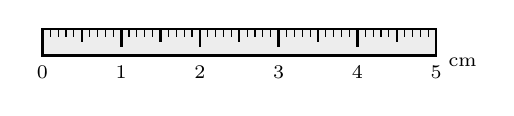
\begin{tikzpicture}[x=1cm, y=1cm, every node/.style={font=\scriptsize, text=black}]
      \draw[black, line width=1.0pt, fill=panelgray] (0,0) rectangle (5.0, 0.34);
      \foreach \m in {0,...,50}{\draw[black, line width=0.4pt] (\m*0.1,0.34)--(\m*0.1,0.24);}
      \foreach \h in {0,0.5,...,5.0}{\draw[black, line width=0.75pt] (\h,0.34)--(\h,0.18);}
      \foreach \c in {0,1,2,3,4,5}{
        \draw[black, line width=1.0pt] (\c,0.34)--(\c,0.11);
        \node[below=0.5pt, font=\scriptsize] at (\c, 0.02) {\en{\c}};
      }
      \node[right=1pt, font=\scriptsize] at (5.0,-0.08) {\en{cm}};
    \end{tikzpicture}
  \end{minipage}
\end{tcolorbox}

\secbox{ផ្នែក ក \enbf{(E2 Explore - POGIL)} ៖ វាស់មុំផ្ចិតលើរង្វង់រួមផ្ចិតខ្នាតពិត និងតារាងសមាមាត្រទ្វេ}{១១ នាទី \en{---} ប្រើរ៉ាប់ព័រទ័រ និងបន្ទាត់ក្រិត}

\noindent
\begin{minipage}[c]{8.80cm}
  \begin{tcolorbox}[enhanced, sharp corners, colback=white, colframe=black, boxrule=0.85pt, boxsep=1pt, top=2pt, bottom=2pt, left=4pt, right=4pt]
    \centering
    {\fontsize{8.1pt}{11pt}\selectfont\textbf{រង្វង់រួមផ្ចិតខ្នាតពិត \en{1:1} ៖ $C_1(O,1.5\unit{cm})$ និង $C_2(O,2.4\unit{cm})$}}\\[1pt]
    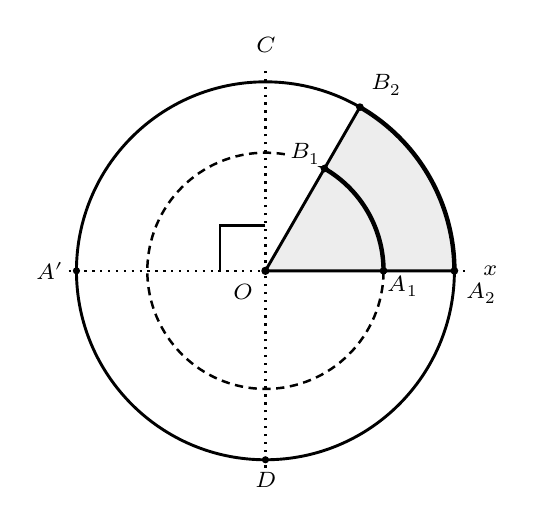
\begin{tikzpicture}[x=1cm, y=1cm, every node/.style={font=\footnotesize, text=black}]
      \coordinate (O) at (0,0);
      \fill[gray!14] (O) -- (0:2.4) arc (0:60:2.4) -- cycle;
      \draw[black, line width=0.9pt, densely dashed] (O) circle (1.5);
      \draw[black, line width=1.05pt] (O) circle (2.4);
      \draw[black, line width=0.85pt, dotted] (-2.5,0) -- (2.6,0) node[right=1pt] {$x$};
      \draw[black, line width=0.85pt, dotted] (0,-2.5) -- (0,2.6) node[above=1pt] {$C$};
      \draw[black, line width=1.05pt] (O) -- (0:2.4) (O) -- (60:2.4);
      \draw[black, line width=1.6pt] (0:1.5) arc (0:60:1.5);
      \draw[black, line width=1.6pt] (0:2.4) arc (0:60:2.4);
      \rightbox[0.24]{0,2.4}{O}{-2.4,0}
      \fill[black] (O) circle (1.5pt) node[below left=1.5pt] {$O$};
      \fill[black] (0:1.5) circle (1.4pt) node[below right=1pt, fill=white, inner sep=0.7pt] {$A_1$};
      \fill[black] (60:1.5) circle (1.4pt) node[above left=1pt, fill=white, inner sep=0.7pt] {$B_1$};
      \fill[black] (0:2.4) circle (1.4pt) node[below right=1pt] {$A_2$};
      \fill[black] (60:2.4) circle (1.4pt) node[above right=1pt] {$B_2$};
      \fill[black] (-2.4,0) circle (1.3pt) node[left=1pt] {$A'$};
      \fill[black] (0,-2.4) circle (1.3pt) node[below=1pt] {$D$};
    \end{tikzpicture}
  \end{tcolorbox}
\end{minipage}%
\hfill
\begin{minipage}[c]{9.80cm}
  \fontsize{8.7pt}{12.6pt}\selectfont
  \textbf{១. ពិសោធន៍វាស់មុំដោយរ៉ាប់ព័រទ័រលើរូបខាងឆ្វេង៖}\\[2pt]
  $\bullet$ មុំផ្ចិតលយ $\ang{A_2OB_2} =$ \blank{1.2cm}$^\circ$ $\Rightarrow$ មុំផ្ចិតឆក $\ang{A_2OB_2} = 360^\circ -$ \blank{1.0cm}$^\circ =$ \blank{1.2cm}$^\circ$ ។\\[2pt]
  $\bullet$ អង្កត់ផ្ចិតពីរកែងគ្នា ($A'A_2 \perp CD$) បង្កើតមុំផ្ចិតកែងចំនួន \blank{0.8cm} មុំ ដែលមុំនីមួយៗស្មើនឹង \blank{1.0cm}$^\circ$ ហើយចែករង្វង់ជា ៤ ធ្នូប៉ុនគ្នាហៅថា \blank{2.2cm} ។\\[2pt]
  $\bullet$ ប្រៀបធៀបធ្នូ $\arc{A_1B_1}$ (លើ $C_1$) និងធ្នូ $\arc{A_2B_2}$ (លើ $C_2$)៖\\
  \hspace*{0.3cm}-- តើធ្នូទាំងពីរស្កាត់ដោយមុំផ្ចិតប៉ុនគ្នាឬទេ? \chkbox\ ប៉ុនគ្នា \quad \chkbox\ មិនប៉ុនគ្នា\\
  \hspace*{0.3cm}-- តើប្រវែងកោងនៃធ្នូណាវែងជាង? \chkbox\ $\arc{A_1B_1}$ \quad \chkbox\ $\arc{A_2B_2}$ \quad \chkbox\ ស្មើគ្នា\\[3pt]
  \begin{tcolorbox}[enhanced, sharp corners, colback=panelgray, colframe=black, boxrule=0.8pt, top=2pt, bottom=2pt, left=4pt, right=4pt]
    \fontsize{8.3pt}{11.5pt}\selectfont
    \textbf{គំនិតគន្លឹះ៖} ធ្នូពីរមាន\textbf{រង្វាស់ដឺក្រេ}ស្មើគ្នា ($60^\circ$) មិនប្រាកដថាមាន\textbf{ប្រវែងគិតជា $\text{cm}$} ស្មើគ្នាទេ លុះត្រាតែរង្វង់ទាំងពីរមាន\textbf{កាំ $r$ ស្មើគ្នា}!
  \end{tcolorbox}
\end{minipage}

\vspace{3pt}
\noindent\textbf{២. បំពេញតារាងសមាមាត្រទ្វេ (\en{Double-Scale Proportional Ratio Table}) ដើម្បីទាញរូបមន្តប្រវែងធ្នូ $l$ ៖}\\[2pt]
{\renewcommand{\arraystretch}{1.48}
\fontsize{8.6pt}{12.2pt}\selectfont
\noindent\begin{tabular}{|L{3.55cm}|C{2.15cm}|C{2.55cm}|C{3.75cm}|C{5.35cm}|}
\hline
\rowcolor{headgray}\textbf{ផ្នែកនៃរង្វង់} & \textbf{មុំផ្ចិតស្កាត់ធ្នូ} & \textbf{ផលធៀបនៃរង្វង់} & \textbf{ប្រវែងធ្នូលើ $C(O, 10\unit{cm})$} & \textbf{រូបមន្តទូទៅលើរង្វង់កាំ $r$} \\
\hline
រង្វង់ពេញ ១ ជុំ (បរិមាត្រ) & $360^\circ$ & $\tfrac{360^\circ}{360^\circ} = 1$ & $P = 2\pi(10) = 20\pi\unit{cm}$ & $P = 2\pi r$ \\
\hline
កន្លះរង្វង់ (អង្កត់ផ្ចិតចែក) & $180^\circ$ & $\tfrac{180^\circ}{360^\circ} = \tfrac{1}{2}$ & $\tfrac{20\pi}{2} =$ \blank{1.8cm}$\unit{cm}$ & $l_{180^\circ} = \tfrac{2\pi r}{2} = \pi r$ \\
\hline
១ កាដ្រង់ (មួយភាគបួនរង្វង់) & $90^\circ$ & $\tfrac{90^\circ}{360^\circ} =$ \blank{1.0cm} & $\tfrac{20\pi}{4} =$ \blank{1.8cm}$\unit{cm}$ & $l_{90^\circ} =$ \blank{2.6cm} \\
\hline
ធ្នូមួយដឺក្រេ ($1^\circ$) & $1^\circ$ & $\tfrac{1^\circ}{360^\circ}$ & $\tfrac{20\pi}{360} =$ \blank{1.8cm}$\unit{cm}$ & $l_{1^\circ} = \tfrac{2\pi r}{360^\circ}$ \\
\hline
\textbf{ធ្នូស្កាត់ដោយមុំផ្ចិត $n^\circ$} & $n^\circ$ & $\tfrac{n^\circ}{360^\circ}$ & $20\pi \times \tfrac{n^\circ}{360^\circ}$ & $l =$ \blank{3.8cm} \\
\hline
\end{tabular}}

\secbox{ផ្នែក ខ \enbf{(E3 Explain)} ៖ សង្ខេបលក្ខណៈទូទៅ រូបមន្តប្រវែងធ្នូ និងធនាគារហេតុផល \enbf{1--5}}{៦ នាទី \en{---} បំពេញនិងកត់ចំណាំ}

\noindent
\begin{minipage}[t]{9.6cm}
  \fontsize{8.9pt}{12.7pt}\selectfont
  $\bullet$ \textbf{ជាទូទៅ (ទំ.១៩៩)៖} ក្នុងរង្វង់មួយ ឬរង្វង់ពីរប៉ុនគ្នា ធ្នូពីរប៉ុនគ្នាស្កាត់ដោយ \blank{2.5cm} ហើយច្រាសមកវិញ កាលណាមុំផ្ចិតពីរប៉ុនគ្នា នោះ \blank{2.5cm} ប៉ុនគ្នា ។\\[2pt]
  $\bullet$ \textbf{សម្គាល់៖} ធ្នូមួយដឺក្រេ ($1^\circ$) ជាធ្នូស្កាត់ដោយមុំផ្ចិត \blank{1.2cm} ។\\[2pt]
  $\bullet$ \textbf{រូបមន្តប្រវែងធ្នូ $n^\circ$ លើរង្វង់កាំ $r$ ៖} $l = \dfrac{2\pi r \times \blank{0.9cm}}{360^\circ} = \dfrac{\pi r \times \blank{0.9cm}}{180^\circ}$ ។
\end{minipage}%
\hfill
\begin{minipage}[t]{9.0cm}
  \begin{tcolorbox}[enhanced, sharp corners, colback=panelgray, colframe=black, boxrule=0.85pt, boxsep=1pt, top=2.5pt, bottom=2.5pt, left=5pt, right=5pt]
    {\muol\fontsize{8.7pt}{12.0pt}\selectfont ធនាគារហេតុផល \enbf{(Warrant Bank)} សម្រាប់យោង៖}\\[1.5pt]
    \fontsize{8.3pt}{11.5pt}\selectfont
    \cnum{1} \textbf{មុំផ្ចិត និងធ្នូស្កាត់៖} រង្វាស់ដឺក្រេនៃធ្នូតូច $\arc{AB}$ ស្មើនឹងមុំផ្ចិត $\ang{AOB}$\\
    \cnum{2} \textbf{កាដ្រង់នៃរង្វង់៖} អង្កត់ផ្ចិតកែងគ្នាចែករង្វង់ជា ៤ កាដ្រង់ ($90^\circ$ ស្មើៗគ្នា)\\
    \cnum{3} \textbf{សមមូលមុំផ្ចិត--ធ្នូ៖} ក្នុង $C(O,r)$ តែមួយ $\ang{AOB}=\ang{COD} \iff \arc{AB}=\arc{CD}$\\
    \cnum{4} \textbf{បរិមាត្ររង្វង់៖} ប្រវែងរង្វង់ពេញ ១ ជុំ ($360^\circ$) គឺ $P = 2\pi r$\\
    \cnum{5} \textbf{រូបមន្តប្រវែងធ្នូ៖} $l = \frac{2\pi r \times n^\circ}{360^\circ}$ (ឯកតាប្រវែងដូចកាំ $r$)
  \end{tcolorbox}
\end{minipage}

\newpage

% ============================================================================
% ទំព័រទី ២៖ E4 លំហាត់គំរូទី១–២ + E5 លំហាត់ប្រតិបត្តិវាស់រ៉ាប់ព័រទ័រ + Exit Check & កិច្ចការផ្ទះ
% ============================================================================
\secbox{ផ្នែក គ \enbf{(E4 Elaborate)} ៖ លំហាត់គំរូទី១ និងទី២ (ទំ.១៩៩--២០០) — គណនាប្រវែងធ្នូនិងត្រួតពិនិត្យឯកតា}{១០ នាទី \en{---} គូស [tracing] និងបំពេញជំហានគណនា}

\noindent
\begin{minipage}[t]{9.25cm}
  \begin{tcolorbox}[enhanced, sharp corners, colback=white, colframe=black, boxrule=0.85pt, top=3pt, bottom=3pt, left=5pt, right=5pt]
    \textbf{លំហាត់គំរូទី១ (ទំ.១៩៩--២០០)៖} នៅលើរង្វង់មានកាំ $r = 10\unit{dm}$ ។ តើធ្នូដែលស្កាត់ដោយមុំផ្ចិត $36^\circ$ មានប្រវែងប៉ុន្មាន $\text{dm}$? ($\pi \approx 3.14$)\\[3pt]
    \begin{minipage}[c]{3.1cm}
      \centering
      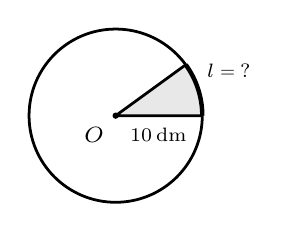
\begin{tikzpicture}[scale=0.88, every node/.style={font=\footnotesize, text=black}]
        \coordinate (O) at (0,0);
        \fill[gray!18] (O) -- (0:1.25) arc (0:36:1.25) -- cycle;
        \draw[black, line width=1.0pt] (O) circle (1.25);
        \draw[black, line width=1.0pt] (O) -- (0:1.25) (O) -- (36:1.25);
        \draw[black, line width=1.6pt] (0:1.25) arc (0:36:1.25);
        \fill[black] (O) circle (1.3pt) node[below left=1pt] {$O$};
        \node[below=1pt, font=\scriptsize] at (0.62,0) {$10\unit{dm}$};
        \node[above right=1pt, font=\scriptsize] at (18:1.22) {$l=?$};
      \end{tikzpicture}
    \end{minipage}%
    \hfill
    \begin{minipage}[c]{5.55cm}
      \fontsize{8.6pt}{13.2pt}\selectfont
      $\bullet$ \textbf{ជំហាន ១ (បរិមាត្រ \cnum{4})៖}\\
      $P = 2\pi r = 2 \times 3.14 \times 10 =$ \blank{1.6cm}$\unit{dm}$\\[2pt]
      $\bullet$ \textbf{ជំហាន ២ (សមាមាត្រប្រវែងធ្នូ \cnum{5})៖}\\
      $360^\circ \longrightarrow P =$ \blank{1.5cm}$\unit{dm}$\\
      $36^\circ \longrightarrow l = \dfrac{\blank{1.5cm} \times 36^\circ}{360^\circ} =$ \blank{1.4cm}$\unit{dm}$\\[2pt]
      $\bullet$ \textbf{ចម្លើយ៖} ប្រវែងធ្នូគឺ $l =$ \blank{1.5cm}$\unit{dm}$ ។
    \end{minipage}
  \end{tcolorbox}
\end{minipage}%
\hfill
\begin{minipage}[t]{9.35cm}
  \begin{tcolorbox}[enhanced, sharp corners, colback=white, colframe=black, boxrule=0.85pt, top=3pt, bottom=3pt, left=5pt, right=5pt]
    \textbf{លំហាត់គំរូទី២ (ទំ.២០០)៖} រង្វង់មានកាំ $r = 15\unit{cm}$ ។ គណនាប្រវែងធ្នូ $80^\circ$ ($\pi = 3.14$) និងផ្ទៀងផ្ទាត់ឯកតាឱ្យបានត្រឹមត្រូវ៖\\[3pt]
    \begin{minipage}[c]{3.1cm}
      \centering
      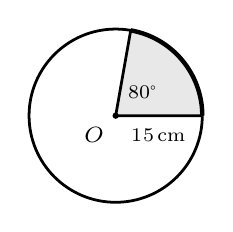
\begin{tikzpicture}[scale=0.88, every node/.style={font=\footnotesize, text=black}]
        \coordinate (O) at (0,0);
        \fill[gray!18] (O) -- (0:1.25) arc (0:80:1.25) -- cycle;
        \draw[black, line width=1.0pt] (O) circle (1.25);
        \draw[black, line width=1.0pt] (O) -- (0:1.25) (O) -- (80:1.25);
        \draw[black, line width=1.6pt] (0:1.25) arc (0:80:1.25);
        \fill[black] (O) circle (1.3pt) node[below left=1pt] {$O$};
        \node[below=1pt, font=\scriptsize] at (0.62,0) {$15\unit{cm}$};
        \node[font=\scriptsize] at (40:0.52) {$80^\circ$};
      \end{tikzpicture}
    \end{minipage}%
    \hfill
    \begin{minipage}[c]{5.65cm}
      \fontsize{8.6pt}{13.2pt}\selectfont
      $\bullet$ \textbf{ជំហាន ១៖} $P = 2 \times 3.14 \times 15 =$ \blank{1.5cm}$\unit{cm}$\\[2pt]
      $\bullet$ \textbf{ជំហាន ២៖} $l = \dfrac{\blank{1.5cm}\unit{cm} \times 80^\circ}{360^\circ}$\\[2pt]
      \hspace*{1.2cm}$= \dfrac{\blank{1.4cm}}{3} \approx$ \blank{1.6cm}$\unit{cm}$\\[2pt]
      $\bullet$ \textbf{ចាប់កំហុសឯកតា៖} ហេតុអ្វីមិនអាចសរសេរ $94.2\unit{dm}$ ក្នុងភាគយក? \blank{2.8cm}
    \end{minipage}
  \end{tcolorbox}
\end{minipage}

\vspace{2pt}
\noindent{\fontsize{8.7pt}{12.5pt}\selectfont\textbf{សំណួរត្រិះរិះ (\en{EIA 30s})៖} នៅក្នុងរូបមន្ត $l = \dfrac{2\pi r \times n^\circ}{360^\circ}$ ហេតុអ្វីបានជាសញ្ញាដឺក្រេ ($^\circ$) រលុបបាត់ ហើយលទ្ធផលនៅសល់តែឯកតាប្រវែងដូចកាំ $r$?\\[2pt]
ចម្លើយ៖ \blank{16.5cm}}

\vspace{3pt}
\secbox{ផ្នែក ឃ \enbf{(E5 Practice)} ៖ លំហាត់ប្រតិបត្តិ (ទំ.២០០) — វាស់មុំផ្ចិតប្រៀបធៀបធ្នូមិនប៉ុនគ្នាលើខ្នាតពិត \enbf{r = 2.00 cm}}{៦.៥ នាទី \en{---} ប្រើរ៉ាប់ព័រទ័រវាស់ផ្ទាល់}

\noindent
\begin{minipage}[c]{6.40cm}
  \begin{tcolorbox}[enhanced, sharp corners, colback=white, colframe=black, boxrule=0.85pt, boxsep=1pt, top=2.5pt, bottom=2.5pt, left=4pt, right=4pt]
    \centering
    {\fontsize{8.1pt}{11pt}\selectfont\textbf{រង្វង់ខ្នាតពិត \en{1:1} ៖ $C(O, 2.00\unit{cm})$ ($\arc{AB} < \arc{CD}$)}}\\[1pt]
    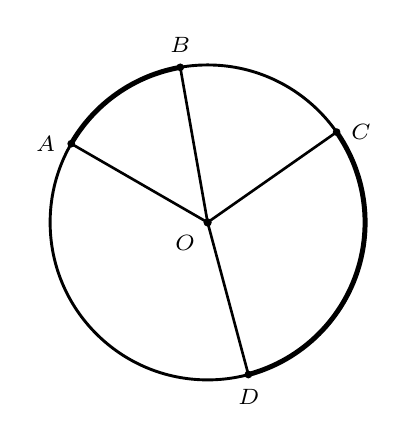
\begin{tikzpicture}[x=1cm, y=1cm, every node/.style={font=\footnotesize, text=black}]
      \coordinate (O) at (0,0);
      \draw[black, line width=1.05pt] (O) circle (2.0);
      \coordinate (A) at (150:2.0);
      \coordinate (B) at (100:2.0);
      \coordinate (C) at (35:2.0);
      \coordinate (D) at (-75:2.0);
      \draw[black, line width=0.95pt] (O) -- (A) (O) -- (B) (O) -- (C) (O) -- (D);
      \draw[black, line width=1.8pt] (B) arc (100:150:2.0);
      \draw[black, line width=1.8pt] (D) arc (-75:35:2.0);
      \fill[black] (O) circle (1.5pt) node[below left=1.5pt] {$O$};
      \fill[black] (A) circle (1.4pt) node[left=2pt] {$A$};
      \fill[black] (B) circle (1.4pt) node[above=2pt] {$B$};
      \fill[black] (C) circle (1.4pt) node[right=2pt] {$C$};
      \fill[black] (D) circle (1.4pt) node[below=2pt] {$D$};
    \end{tikzpicture}
  \end{tcolorbox}
\end{minipage}%
\hfill
\begin{minipage}[c]{12.20cm}
  \textbf{ប្រតិបត្តិ (ទំ.២០០)៖} នៅលើរង្វង់ $C(O, 2.00\unit{cm})$ ខាងឆ្វេង គេមានធ្នូតូចពីរមិនប៉ុនគ្នាគឺ $\arc{AB} < \arc{CD}$ ។ ចូរប្រើរ៉ាប់ព័រទ័រវាស់មុំផ្ចិតទាំងពីរ រួចគណនាប្រវែងធ្នូ ($\pi \approx 3.14$)៖\\[3pt]
  {\renewcommand{\arraystretch}{1.38}
  \fontsize{8.7pt}{12.5pt}\selectfont
  \begin{tabular}{|C{2.4cm}|C{3.3cm}|C{5.5cm}|}
    \hline
    \rowcolor{headgray}\textbf{ធ្នូនៃរង្វង់} & \textbf{មុំផ្ចិតដែលវាស់បាន} & \textbf{គណនាប្រវែងធ្នូ $l = \frac{2\pi r \cdot n^\circ}{360^\circ}$} \\
    \hline
    ធ្នូតូច $\arc{AB}$ & $\ang{AOB} =$ \blank{1.2cm}$^\circ$ & $l_{AB} =$ \blank{3.6cm}$\unit{cm}$ \\
    \hline
    ធ្នូតូច $\arc{CD}$ & $\ang{COD} =$ \blank{1.2cm}$^\circ$ & $l_{CD} =$ \blank{3.6cm}$\unit{cm}$ \\
    \hline
  \end{tabular}}\\[4pt]
  $\bullet$ \textbf{ប្រៀបធៀបមុំផ្ចិត៖} $\ang{AOB}$ \blank{0.9cm} $\ang{COD}$ (ដាក់សញ្ញា $<, >$ ឬ $=$) ។\\[2pt]
  $\bullet$ \textbf{សេចក្ដីសន្និដ្ឋាន៖} នៅក្នុងរង្វង់តែមួយ បើធ្នូតូច $\arc{AB} < \arc{CD}$ នោះមុំផ្ចិតស្កាត់ធ្នូទាំងពីរផ្ទៀងផ្ទាត់ \blank{3.2cm} ហើយប្រវែងធ្នូ $l_{AB}$ \blank{0.9cm} $l_{CD}$ ។
\end{minipage}

\vspace{3pt}
\secbox{ផ្នែក ង \enbf{(E5 Exit Check \& Homework)} ៖ រង្វាយតម្លៃរហ័ស \enbf{A--D} និងកិច្ចការផ្ទះ (ទំ.២០៤)}{៣.៥ នាទី + កិច្ចការផ្ទះ}

\noindent\textbf{១. គូសសញ្ញា \ding{51} ក្នុងប្រអប់ \chkbox\ ត្រូវ ឬ \chkbox\ ខុស ព្រមទាំងបញ្ជាក់លេខហេតុផល (\cnum{1}--\cnum{5})៖}\\[2.5pt]
{\renewcommand{\arraystretch}{1.30}
\noindent\begin{tabular}{|C{0.7cm}|L{11.7cm}|C{2.9cm}|C{2.4cm}|}
\hline
\rowcolor{headgray}\textbf{កាត} & \textbf{អំណះអំណាងវិនិច្ឆ័យ} & \textbf{ជម្រើស} & \textbf{លេខហេតុផល} \\
\hline
\textbf{A} & អង្កត់ផ្ចិតពីរកែងគ្នាចែករង្វង់ជា ៤ កាដ្រង់ ដែលកាដ្រង់នីមួយៗមានរង្វាស់មុំផ្ចិត $90^\circ$ ។ & \chkbox\ ត្រូវ \quad \chkbox\ ខុស & \blank{1.5cm} \\
\hline
\textbf{B} & រង្វង់ពីរមានកាំ $r_1 = 4\unit{cm}$ និង $r_2 = 8\unit{cm}$ នោះធ្នូ $60^\circ$ នៃរង្វង់ទាំងពីរមានប្រវែងស្មើគ្នា ។ & \chkbox\ ត្រូវ \quad \chkbox\ ខុស & \blank{1.5cm} \\
\hline
\textbf{C} & ធ្នូដែលស្កាត់ដោយមុំផ្ចិត $60^\circ$ មានប្រវែងស្មើនឹង $\frac{1}{6}$ នៃបរិមាត្ររង្វង់ ($l = \frac{\pi r}{3}$) ។ & \chkbox\ ត្រូវ \quad \chkbox\ ខុស & \blank{1.5cm} \\
\hline
\textbf{D} & នៅក្នុងរង្វង់ $C(O,r)$ តែមួយ បើមុំផ្ចិតពីរប៉ុនគ្នា នោះធ្នូដែលស្កាត់ដោយមុំផ្ចិតទាំងពីរក៏ប៉ុនគ្នាដែរ ។ & \chkbox\ ត្រូវ \quad \chkbox\ ខុស & \blank{1.5cm} \\
\hline
\end{tabular}}

\vspace{4pt}
\begin{tcolorbox}[enhanced, sharp corners, colback=panelgray, colframe=black, boxrule=0.95pt, top=3pt, bottom=3pt, left=6pt, right=6pt]
  {\muol\fontsize{9.0pt}{13pt}\selectfont កិច្ចការផ្ទះ (សៀវភៅសិក្សាគោល ទំព័រ ២០៤ ៖ លំហាត់ទី១ + លំហាត់អនុវត្តប្រវែងធ្នូ)}\\[2pt]
  \fontsize{8.7pt}{12.7pt}\selectfont
  $\bullet$ \textbf{១. លំហាត់ទី១ (ទំ.២០៤)៖} គេឱ្យរង្វង់ $C(O,r)$ និងអង្កត់ធ្នូ $AB$ ដែលមុំ $\ang{OAB} = 25^\circ$ ។ ចូរគណនារង្វាស់ដឺក្រេនៃធ្នូតូច $\arc{AB}$ (\textit{តម្រុយ៖ គូសកាំ $OA, OB$ បាន $\tri{OAB}$ សមបាទកំពូល $O \Rightarrow \ang{OBA}=\ang{OAB}=25^\circ$ រួចរកមុំផ្ចិត $\ang{AOB}$}) ។\\[1.5pt]
  $\bullet$ \textbf{២. អនុវត្ត៖} បើរង្វង់ក្នុងលំហាត់ទី១ ខាងលើមានកាំ $r = 18\unit{cm}$ ចូរគណនាប្រវែងធ្នូតូច $\arc{AB}$ គិតជា $\text{cm}$ (យក $\pi \approx 3.14$) ។
\end{tcolorbox}

\end{document}
